\chapter{Desarrollo de la aplicación}

\section{Generalidades}

En esta sección se presentan generalidades del diseño de la aplicación. Se explica el por qué se siguió el modelo MVC tradicional y los navegadores con los cuales se garantiza que la aplicación sea completamente funcional.

\subsection{Modelo MVC}

El patrón de diseño MVC es uno de los más populares para la creación de aplicaciones, tanto de escritorio como web. Esto debido a que permite que los componentes de la arquitectura del software puedan variar de manera casi independiente y aún así seguir proveyendo una correcta funcionalidad a la aplicación. De esta manera, no solo se puede hacer un diseño limpio y fácil de entender y depurar, sino que es más fácil realizar actualizaciones y darles mantenimiento, ya que si algo falla, es bastante evidente cual de los componentes es el que está fallando. Además, el MVC facilita la programación orientada a objetos, paradigma que ya se tiene en HTML5 con los DOM, por lo que es apropiado utilizarlo. \\

Para seguir este patrón las divisiones se realizaron de la siguiente manera:

\begin{enumerate}
\item Los Views están compuestos por los diferentes archivos en el lenguaje HTML5 que le permiten al usuario visualizar en su navegador la aplicación y poder interactuar con la misma.

\item Los Controllers son varios archivos en JavaScript, utilizando el framework AngularJS, que permiten dar funciones específicas a las interacciones que tiene el usuario con los Views. Los controllers envían peticiones HTTP, como los son los POSTs, GETs, PUTs para modificar los contenidos del Model.

\item El Model se realizó utilizando el framework LoopBack de Stronloops y algunas funciones del NodeJS. Además la persistencia de los datos se realiza haciendo uso de una base de datos en MongoDb.  

\end{enumerate}

\subsection{Navegadores}

El diseño de aplicaciones web con lleva un reto: se debe de realizar tomando en cuenta las diferentes tecnologías que utilizan los navegadores comerciales más populares que se usan en la actualidad: Chrome, Firefox, Iceweasel, Opera, Internet Explorer de Microsoft (fuera de soporte y próximamente se utilizará Edge) y Safari en Mac OS X.\\

Para el desarrollo de la aplicación de este proyecto, se seleccionaron los dos navegadores más utilizados en la actualidad, Firefox y Chrome. Se diseñó y corroboró el funcionamiento en estos dos navegadores pero no se garantiza el completo funcionamiento de la aplicación en otros navegadores, con la excepción de Iceweasel, que es la versión de software libre de Firefox, presente en los sistemas operativos Debian, ya que para este navegador también se realizaron pruebas y funciona de igual manera que Firefox.

\section{Frontend}

Para el desarrollo del frontend de la aplicación se eligió utilizar HTML5, CSS3 y AngularJS. Esto debido a las funcionalidades predeterminadas que tiene HTML5 como cargar videos, realizar streaming de video y los elementos como el canvas. CSS3 es el que le brinda el estilo a los elementos del documentos permitiendo personalizar los colores, fuente, posiciones y otras características de la página web, dándole así la apariencia deseada. Finalmente Angular permite darle las características dinámicas que requiere la interfaz para obtener una buena experiencia de usuario.\\

\subsection{Consideraciones Generales}

Como una consideración general en todos los modos de operación de la aplicación, para operar sobre los cuadros del video se utiliza el elemento video de las librerías de HTML5 y se utiliza la propiedad del video \emph{currentTime} al cual se puede escribir para poner un valor de punto flotante en segundos para moverse a ese punto exacto del video. Sabiendo la duración del video en segundos y la tasa de FPS, se multiplican para obtener la cantidad de cuadros totales. Para avanzar cuadro por cuadro se le suma a \emph{currentTime} + $1/\text{FPS}$, para retroceder cuadro a cuadro se le resta, y para ir a un cuadro específico solo se iguala a $\frac{ \text{i}}{FPS}$, donde i es el número de cuadro al que se quiere ir, y con dicha división se obtiene el tiempo actual en segundos al que se quiere ir. 

En AngularJS, como se explicó en el marco teórico se tienen diferentes formas de llevar a cabo las funciones del fronted. Entre ellas están los controllers que son la principal fuente de interacción con el usuario y los services, que son ayudan a tener una funcionalidad general en todos los views de una aplicación. Por esta razón el menu principal se realizó como un service y los demás métodos de interacción con el usuarios se pusieron dentro de las clases de controllers.

La estructura del frontend cuenta con los siguientes componentes:

\begin{enumerate}
\item Controllers:
	\begin{enumerate}
		\item View1Ctrl: controller para el modo de operación de segmentación temporal.
		\item View2Ctrl: controller para el modo de operación de trayectorias de objetos.
		\item View3Ctrl: controller para el modo de operación de segmentación por contornos.
		\item View4Ctrl: controller para el modo de operación de segmentación semántica
	\end{enumerate}
\item Services:
	\begin{enumerate}
		\item LeftMenu: service presente en todos los modos de operación para tener acceso al menu principal de la aplicación.
	\end{enumerate}

\item App: módulo principal de la aplicación. Es el que realiza el routing de las peticiones realizadas al servidor y lo redirige al controller indicado, el cual actualizará el view de la manera indicada para que se visualice la información de manera correcta.

\end{enumerate}


Siguiendo el modelo MVC, en esta parte del diseño se abarcan los componentes tanto de los Views como los Controllers. Estos se dividen en las siguientes secciones:\\

\begin{itemize}
\item Menu principal: Service LeftMenu, es un controller en el patrón MVC.

\item Interfaces: son cuatro, y todas tienen elementos tanto de Views, como los son archivos HTML5 y CSS de cada uno, y tienen los Controllers respectivos para las funcionalidades que se exponen más adelante Las interfaces son las siguientes:

 \begin{enumerate}
		\item Interfaz para la segmentación temporal
		\item Interfaz para las trayectorias de objetos
		\item Interfaz para la segmentación de contornos 
		\item Interfaz para la segmentación semántica
\end{enumerate}


\end{itemize}

A continuación se describe el menu principal y cada una de estas interfaces de frontend.

\subsection{Menu Principal}

Para contar con un menú principal que no interfiriera con el espacio necesario para poder visualizar los videos, y realizar las anotaciones de una manera cómoda y ordenada; se decidió hacer un menú deslizante en la parte izquierda de la pantalla. El menú se puede mostrar u ocultar haciendo click sobre el nombre de la aplicación. En la Figura \ref{fig:menuFull} se muestra como se observaría la interfaz del programa con el menú principal abierto y en la Figura \ref{fig:mainmenu} se hace un acercamiento al menú para que se puede apreciar bien el contenido del mismo. 

Desde este menú se varía el modo de operación de la aplicación, por lo que cada vez que se acceda a él y se seleccione un modo diferente se cargan las configuraciones predeterminadas para dicho modo y la interfaz se adecua de manera apropiada.

\begin{figure}
	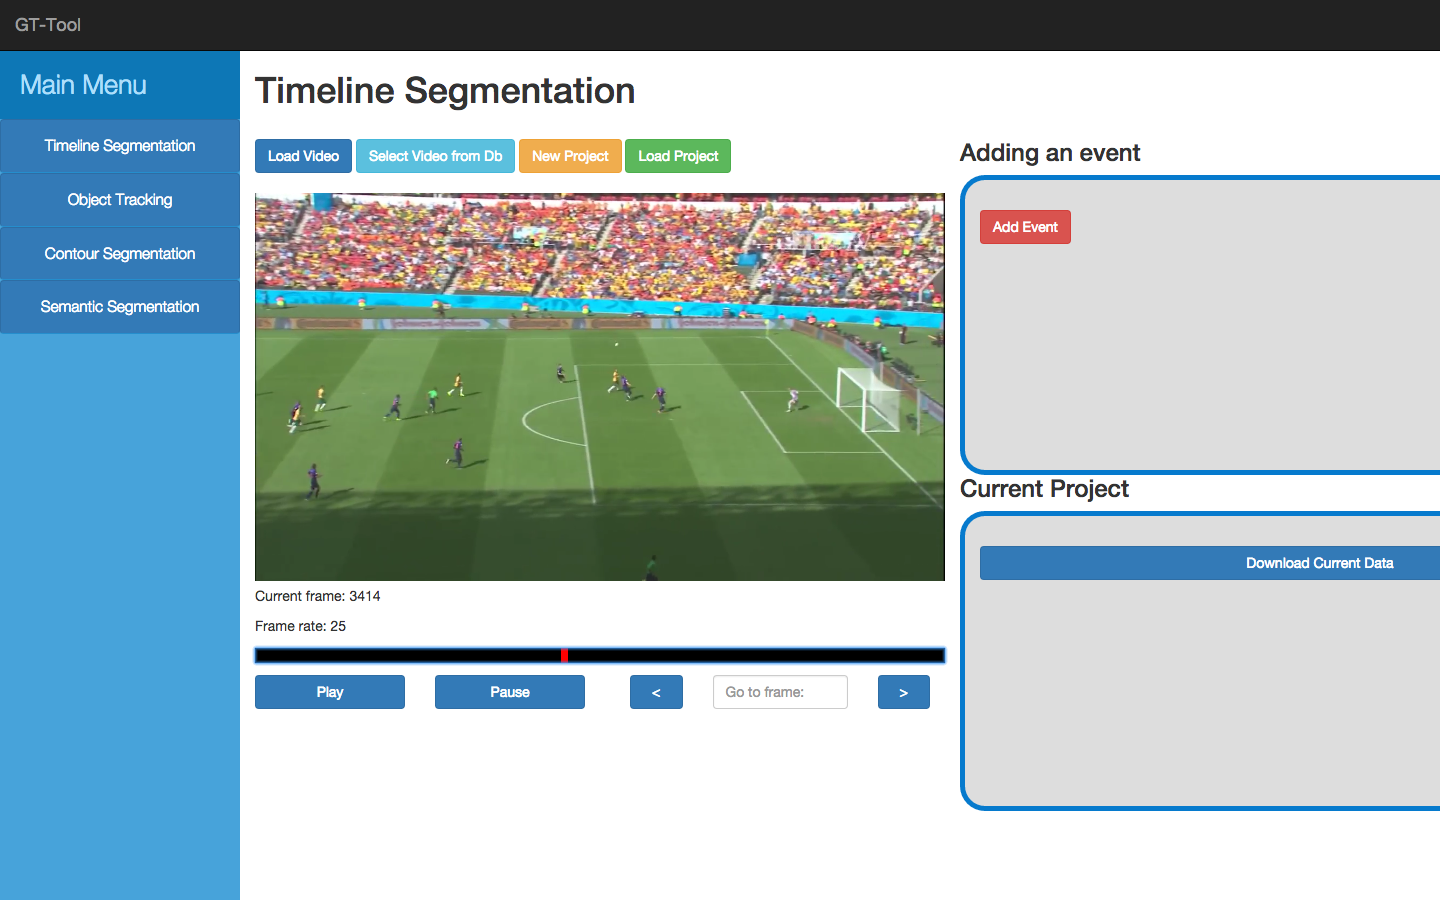
\includegraphics[width=\linewidth]{images/menuFull}
	\caption{Menú principal deslizante desde la izquierda} \label{fig:menuFull}
\end{figure}

\begin{figure}
	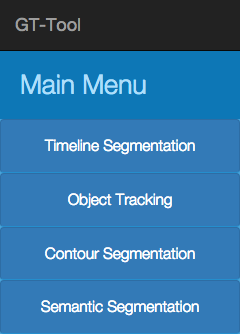
\includegraphics[width=0.35\linewidth]{images/mainmenu}
	\caption{Acercamiento del menú principal} \label{fig:mainmenu}
\end{figure}

Además cada una de las interfaces cuenta con los mismos botones superiores que realizan las funciones de cargar un video local, cargar un video que se haya hecho disponible desde el servidor, cargar un proyecto anterior o crear un nuevo proyecto. Toda está información de proyectos nuevos se almacena directamente en la base de datos del servidor. Cada uno de estos botones despliega las ventanas mostradas en la Figura \ref{fig:loads}.

\begin{figure}
	
	\centering
	\begin{subfigure}[t]{0.48\textwidth}
		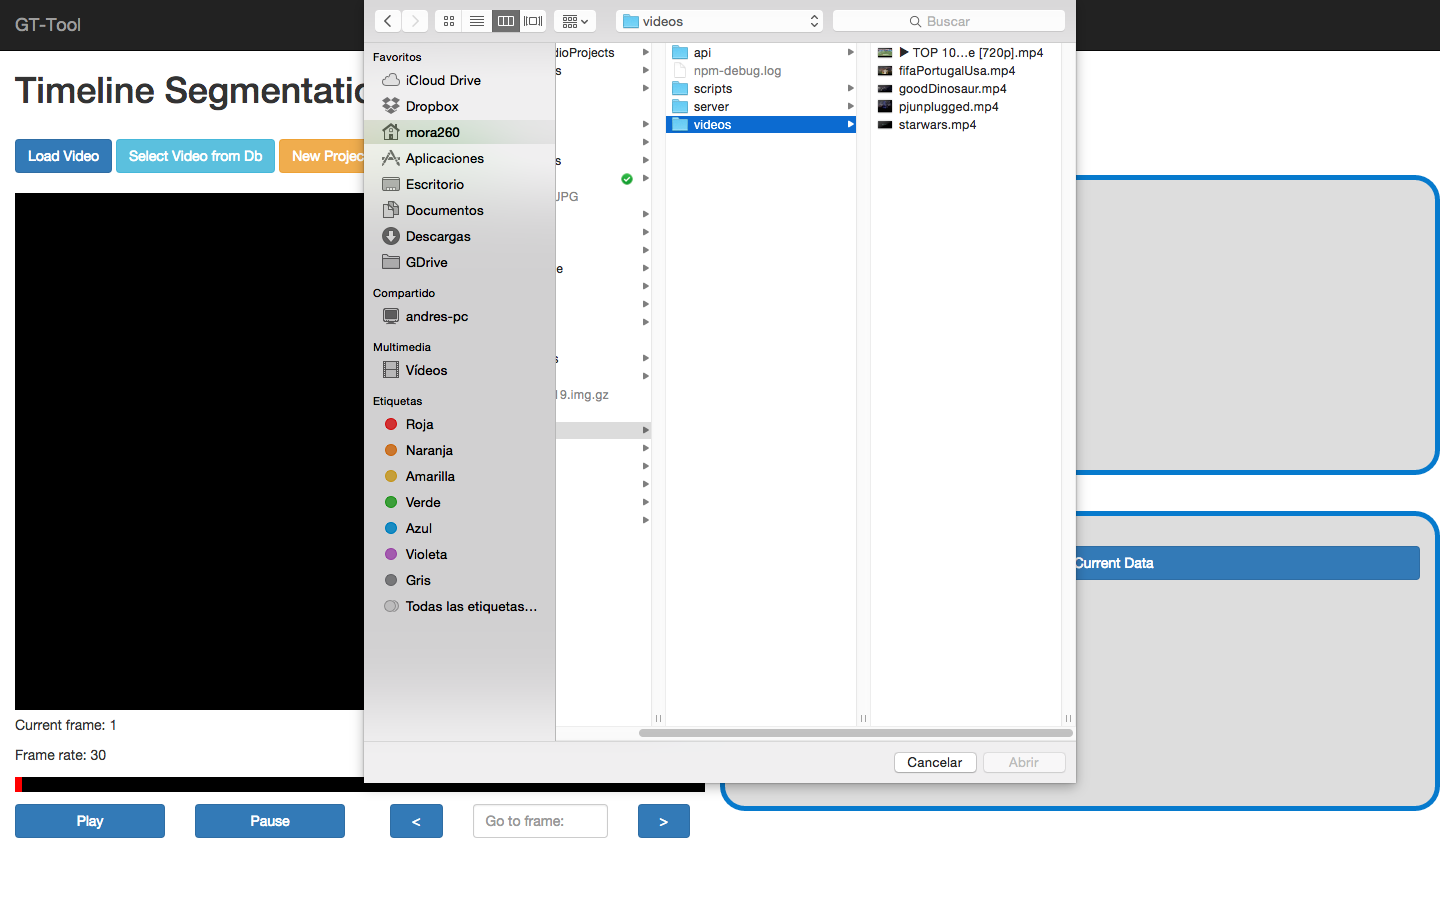
\includegraphics[width=\textwidth]{images/videoL}
		\caption{Selección de videos locales}
		\label{fig:v1}
	\end{subfigure}
	~ %add desired spacing between images, e. g. ~, \quad, \qquad, \hfill etc. 
	%(or a blank line to force the subfigure onto a new line)
	\begin{subfigure}[t]{0.48\textwidth}
		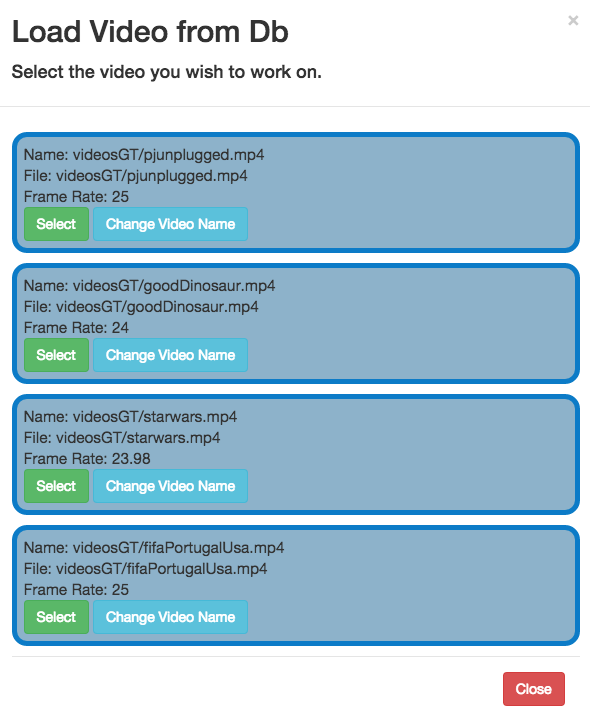
\includegraphics[width=\textwidth]{images/videos}
		\caption{Selección de videos desde la base de datos}
		\label{fig:v2}
	\end{subfigure}
	~ %add desired spacing between images, e. g. ~, \quad, \qquad, \hfill etc. 
	%(or a blank line to force the subfigure onto a new line)
	\begin{subfigure}[t]{0.48\textwidth}
		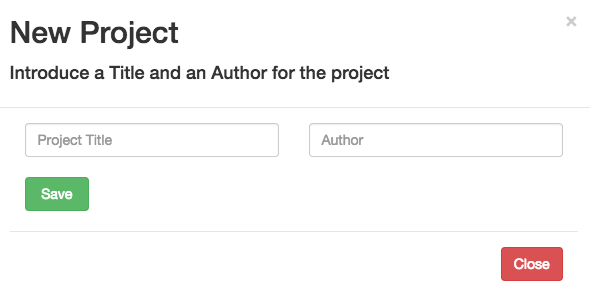
\includegraphics[width=\textwidth]{images/proyectos}
		\caption{Creación de un proyecto nuevo}
		\label{fig:v3}
	\end{subfigure}
	~ %add desired spacing between images, e. g. ~, \quad, \qquad, \hfill etc. 
	%(or a blank line to force the subfigure onto a new line)
	\begin{subfigure}[t]{0.48\textwidth}
		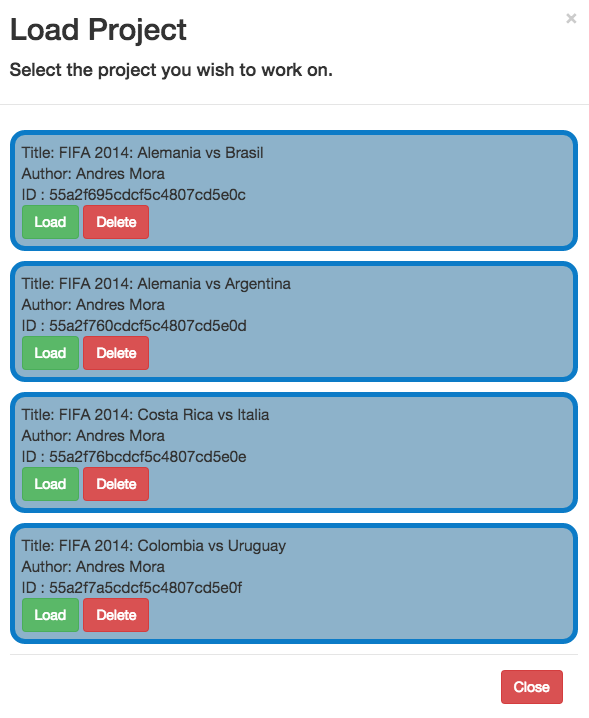
\includegraphics[width=\textwidth]{images/proyectoL}
		\caption{Menú para manipular datos previos y descargar}
		\label{fig:v4}
	\end{subfigure}
	\caption{Cargar proyectos desde la base de datos}\label{fig:loads}
	
\end{figure}

Además para los modos segmentación de contornos y trayectoria de objetos, se incluyó un selector de color para poder variar los tonos con lo que se hacen las anotaciones espaciales. Este selector se puede visualizar en la Figura \ref{fig:colores}, y el mismo aparece cada vez que se va a agregar un nuevo seguimiento o un nuevo contorno a la lista del video.


\begin{figure}
	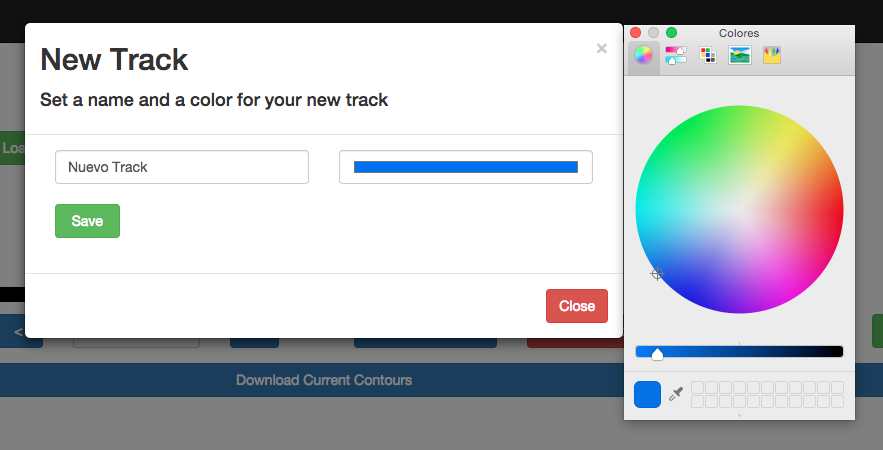
\includegraphics[width=0.7\linewidth]{images/colores}
	\caption{Selector de colores para los modos de trayectorias y contornos} \label{fig:colores}
\end{figure}

A continuación se describe las interfaces de los diferentes modos de operación de manera detallada.

\subsection{Interfaz de segmentación temporal}

El primero de los modos de operación es el de segmentación temporal. Su interfaz completa se puede apreciar en la Figura \ref{fig:tempFull}. En esta se visualiza el video en la parte izquierda de la ventana principal. A la derecha se tiene dos ventanas secundarias.\\

\begin{figure}
	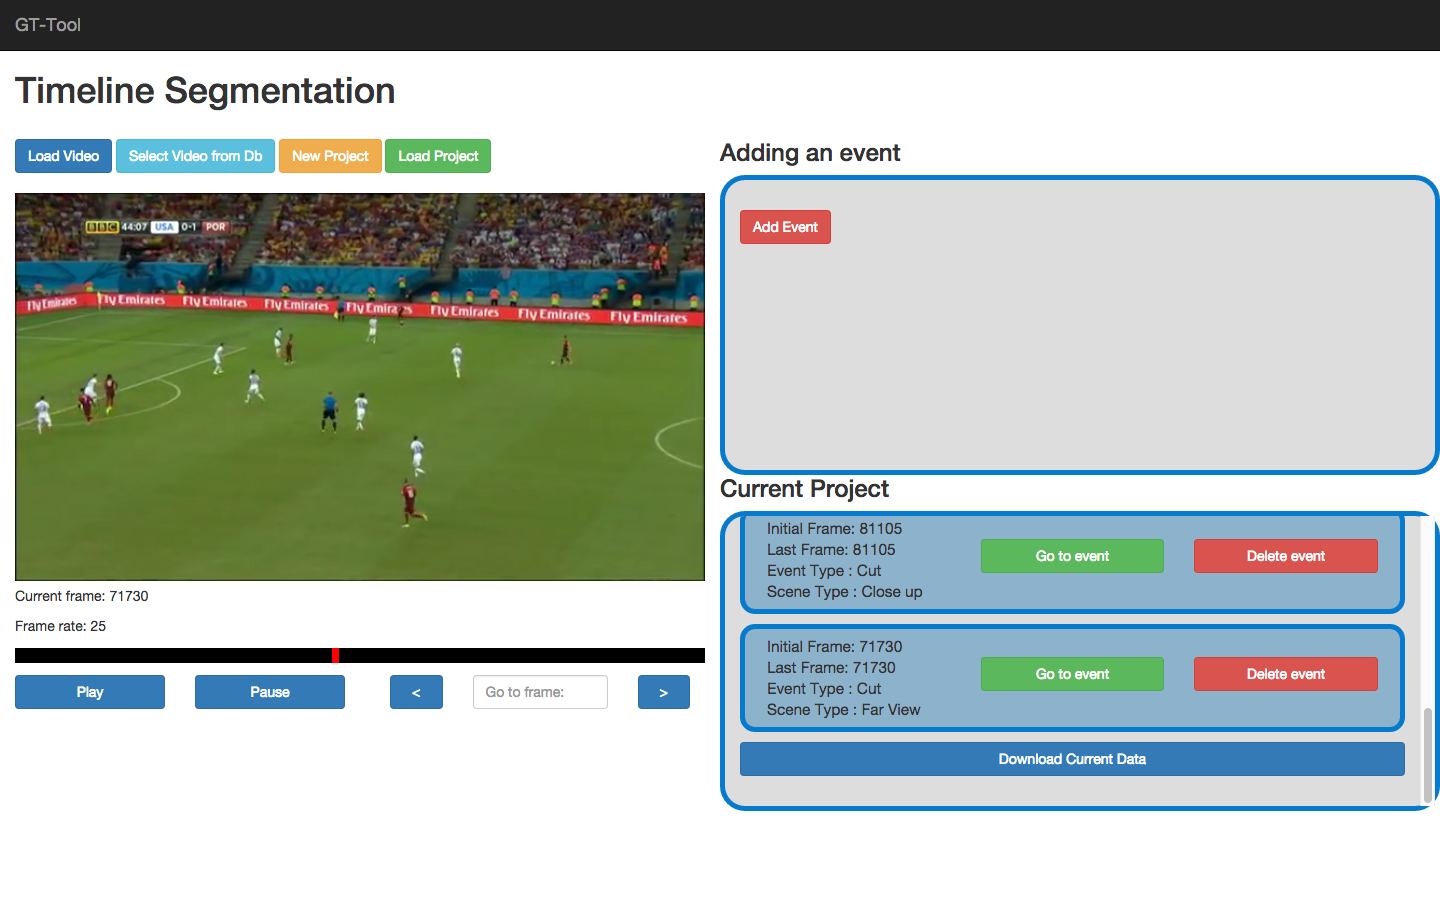
\includegraphics[width=\linewidth]{images/tempFull}
	\caption{Interfaz de la segmentación temporal completa} \label{fig:tempFull}
\end{figure}

En la superior aparece el botón de añadir evento, el cual inicia una secuencia de eventos que le permite al usuario seleccionar el tipo de evento que ha presentando. Se inicia seleccionando el cuadro en el que ha ocurrido, luego se elige el tipo de transición, después el cuadro final de la transición y por último el tipo de escena que inicia luego de finalizada la transición. En el caso especial de un corte que el cuadro inicial y el final son el mismo, se omite el paso de seleccionar cuadro final. Finalmente se presenta al usuario un cuadro resumen con los datos que el mismo ingresó y con el botón de guardar, se añade el evento a la base de datos. En la capturas de pantalla organizadas en la Figura   \ref{fig:temptemp} se muestra el proceso descrito anteriormente de manera visual. En la imagen \ref{fig:temp1} es el primer paso luego de seleccionar añadir un evento. Se avanza a \ref{fig:temp2} y se agrega el tipo de transición, finalmente en \ref{fig:temp3} se elije el tipo de escena que se inició. En \ref{fig:temp4} se puede observar el resumen de datos que se le muestra al usuario antes de grabar el evento creado. \\

\begin{figure}
	
	\centering
	\begin{subfigure}[b]{0.7\textwidth}
		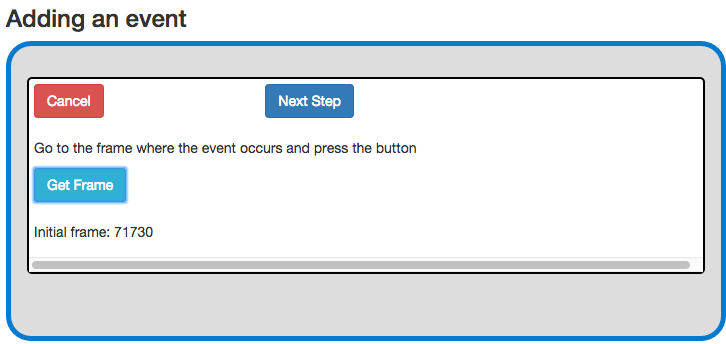
\includegraphics[width=\textwidth]{images/temp1}
		\caption{Selección de primer cuadro}
		\label{fig:temp1}
	\end{subfigure}
	~ %add desired spacing between images, e. g. ~, \quad, \qquad, \hfill etc. 
	%(or a blank line to force the subfigure onto a new line)
	\begin{subfigure}[b]{0.7\textwidth}
		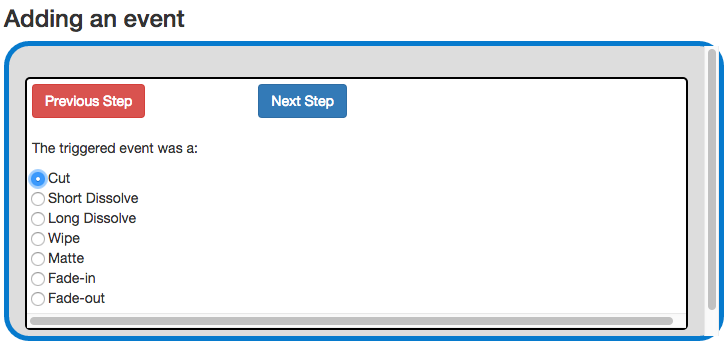
\includegraphics[width=\textwidth]{images/temp2}
		\caption{Selección del tipo de transición}
		\label{fig:temp2} 
	\end{subfigure}
	~ %add desired spacing between images, e. g. ~, \quad, \qquad, \hfill etc. 
	%(or a blank line to force the subfigure onto a new line)
	\begin{subfigure}[b]{0.7\textwidth}
		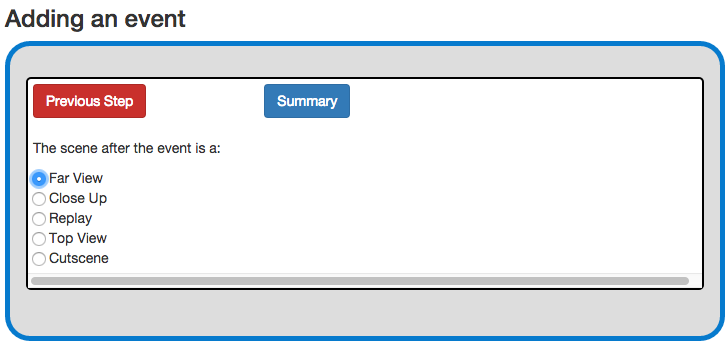
\includegraphics[width=\textwidth]{images/temp3}
		\caption{Selección del tipo de datos antes de guardar}
		\label{fig:temp3}
	\end{subfigure}
	~ %add desired spacing between images, e. g. ~, \quad, \qquad, \hfill etc. 
	%(or a blank line to force the subfigure onto a new line)
	\begin{subfigure}[b]{0.7\textwidth}
		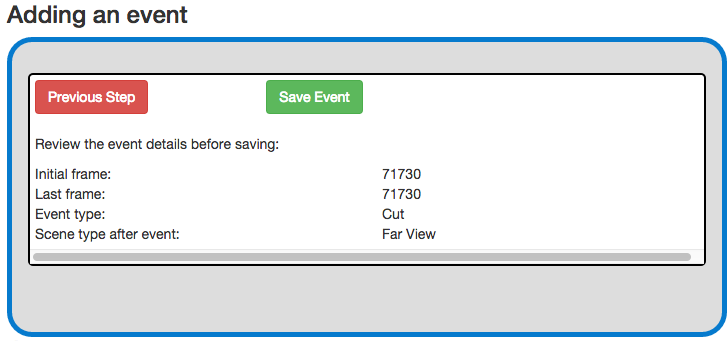
\includegraphics[width=\textwidth]{images/temp4}
		\caption{Resumen para el usuario antes de almacenar el dato.}
		\label{fig:temp4}	
	\end{subfigure}
	\caption{Detalle del funcionamiento en el módulo de agregar evento a la segmentación temporal}\label{fig:temptemp}
	
\end{figure}

En la inferior aparece una pequeña ventana de visualización de todos los eventos que han sido agregados en dicho proyecto. En esta ventana se puede tomar dos decisiones por cada evento: ir al cuadro inicial en el que ocurren, o eliminarlo de la base de datos. Dicha se ventana se puede apreciar le Figura \ref{fig:temp5} De esta manera se pueden agregar y eliminar eventos de un proyecto. Al final de la visualización de todos los eventos, se presenta un botón de descarga, el cual a la hora de presionarlo, descarga a la computadora local un archivo de formato JSON con todas las anotaciones realizadas hasta el momento.\\

\begin{figure}
	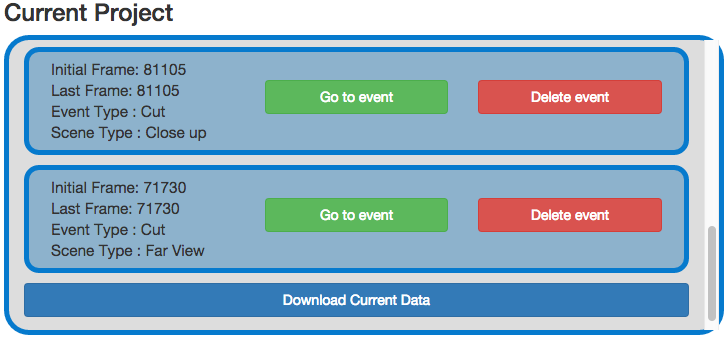
\includegraphics[width=0.7\linewidth]{images/temp5}
	\caption{Panel para eliminar segmentaciones previas o para ir a la segmentación seleccionada.} \label{fig:temp5}
\end{figure}


Para este modo de operación, el programa graba constantemente de manera automática. Esto porque se evita la perdida de datos en cualquier eventualidad y porque al poder añadir y borrar de manera sencilla, no afecta que el programa guarde y actualice la base de datos de manera automática.


\subsection{Interfaz de trayectorias}

El modo para describir trayectorias varía su interfaz de gran manera en comparación a la segmentación temporal, esto debido a que ahora no solo se tiene información en una dimensión (el tiempo). En este modo se tiene información en tres dimensiones: en el eje $x$ de la imagen, en el $y$ y en el $tiempo$. Por esta razón la complejidad y opciones de la interfaz incrementan. Ahora no se tienen los dos paneles a la derecha. El video toma el 100\% de su tamaño en la interfaz de la aplicación. Es decir, un video de 1920x1080 se desplegará con estas dimensiones sin importar la resolución actual de la pantalla. Se habilitan barras de desplazamiento para la completa visualización del video si la dimensión de este es mayor a la resolución del monitor. Esta decisión de diseño se tomó ya que si se está realizando seguimiento de objetos, lo mejor es que la precisión de pixeles sea grande, y la mejor manera para esto es que la proporción entre el video original y el que realmente se despliega en pantalla sea de 1 a 1. La interfaz general de este modo se aprecia en la Figura \ref{fig:objFull}.\\

\begin{figure}
	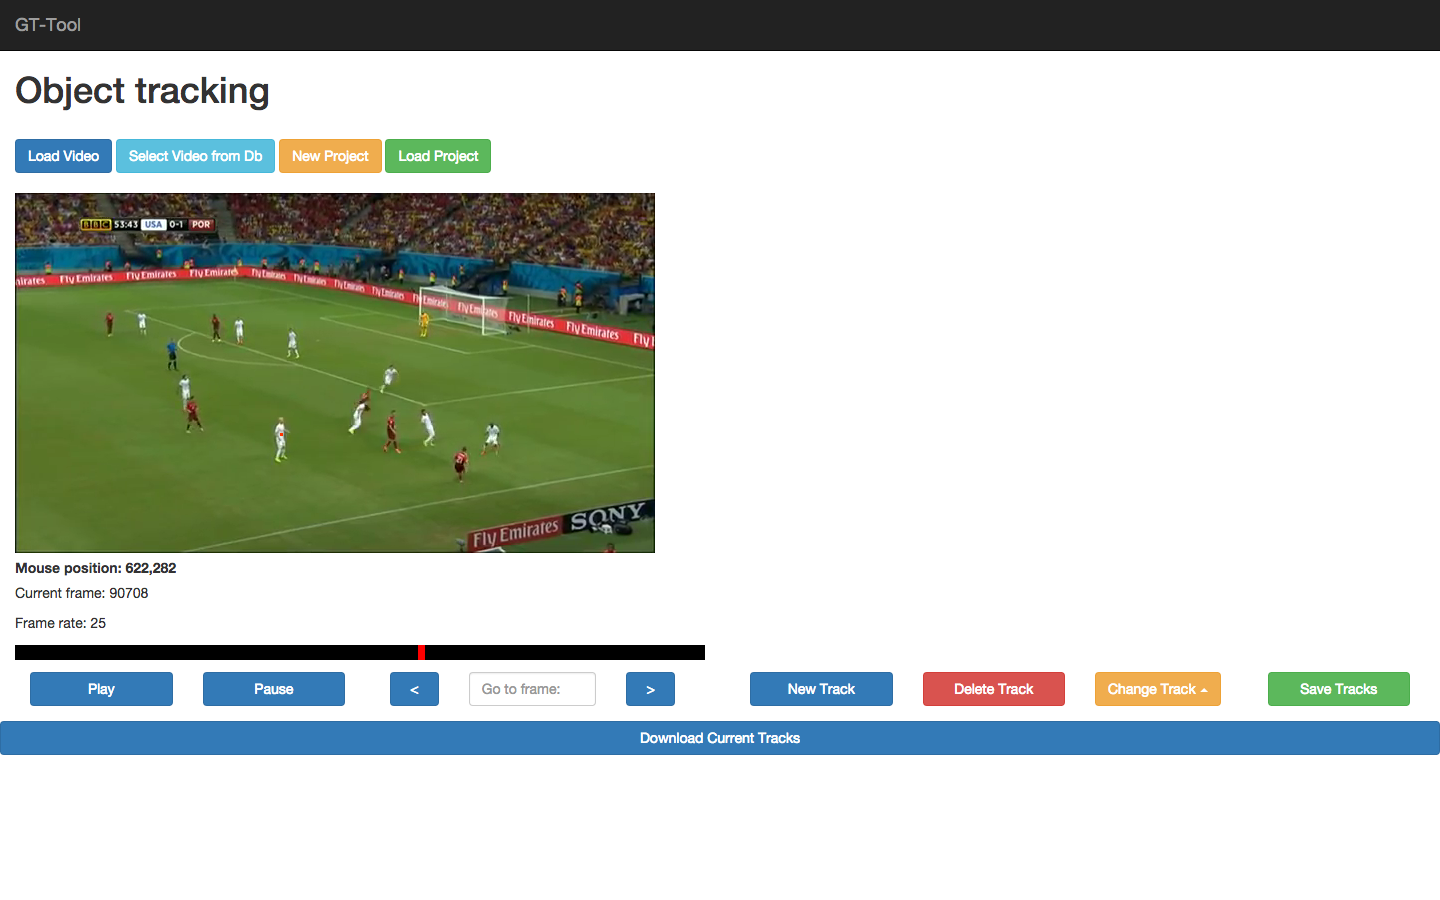
\includegraphics[width=\linewidth]{images/objFull}
	\caption{Interfaz de trayectorias completa} \label{fig:objFull}
\end{figure}

El menú para agregar anotaciones al video en este modo se detalla en la Figura \ref{fig:objobj}. En \ref{fig:obj1} se muestran los botones para agregar una nueva trayectoria, para eliminar la trayectoria actual, para cambiar la trayectoria actual y para salvar todo el contenido editado hasta el momento en la base de datos. En \ref{fig:obj2} se muestra como se selecciona con un drop menu el nombre de la trayectoria que se quiere continuar editando. Finalmente en la Figura \ref{fig:obj3} se muestra como se ve el video luego de que se agrega una punto de trayectoria a algún objeto.\\

Debido a su naturaleza, en este modo no se permite agregar más de un punto por cuadro. Ya que cada uno de estos representa un momento en el tiempo y un objeto no puede estar en dos posiciones a la vez. Por esta razón, el agregar un segundo punto en el mismo cuadro se bloquea a menos de que el el punto sea previamente eliminado. De igual manera, este modo tiene un botón grande en la parte inferior que permite poder descargar las trayectorias que han sido cargadas o que se han trazado en el proyecto actual.\\

A diferencia del modo de operación anterior, para grabar los cambios realizados en las trayectorias de los objetos, es necesario pulsar el botón de grabar. Esto debido a que se agrega un punto por cada cuadro, por lo que no se quiere estar escribiendo tantas veces a la base de datos. El usuario es responsable por guardar los avances antes de cerrar la aplicación. Si se crea una nueva trayectoria o se cambia a otra, en estos casos el programa si genera un autoguardado en la base de datos del contenido de la trayectoria que se está dejando antes de cargar o crear uno diferente.

\begin{figure}
	
	\centering
	\begin{subfigure}[b]{\textwidth}
		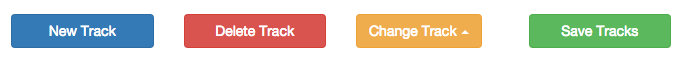
\includegraphics[width=\textwidth]{images/obj1}
		\caption{Menú para administrar las trayectorias}
		\label{fig:obj1}
	\end{subfigure}
	~ %add desired spacing between images, e. g. ~, \quad, \qquad, \hfill etc. 
	%(or a blank line to force the subfigure onto a new line)
	\begin{subfigure}[b]{0.18\textwidth}
		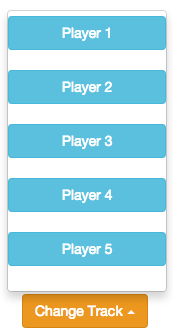
\includegraphics[width=\textwidth]{images/obj2}
		\caption{Selección de trayectoria actual}
		\label{fig:obj2}
	\end{subfigure}
	\qquad \qquad \qquad ~ %add desired spacing between images, e. g. ~, \quad, \qquad, \hfill etc. 
	%(or a blank line to force the subfigure onto a new line)
	\begin{subfigure}[b]{0.18\textwidth}
		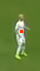
\includegraphics[width=\textwidth]{images/obj3}
		\caption{Rastreo de la posición del objeto}
		\label{fig:obj3}
	\end{subfigure}
	\caption{Elementos de la interfaz para rastreo}\label{fig:objobj}
	
\end{figure}

\clearpage

\subsection{Interfaz de segmentación de contornos}

La segmentación espacial a partir de contornos comparte la misma interfaz que el modo anterior. Esto debido a que la visualización de información relevante es también en las dimensiones de $x$, $y$, y $t$. A diferencia del anterior, en este modo si se puede agregar más de un punto por cuadro, de hecho, la funcionalidad recae en que se tomen todos los pixeles por lo cuales se mueve el puntero del ratón mientras el botón izquierdo del mouse este presionado.

Como se puede apreciar en la Figura \ref{fig:contourFull} y comparando con la Figura \ref{fig:objFull} se ve que ambas interfaces son las mismas. Ahora bien, si se observa la Figura \ref{fig:contour1} se ve que el contorno realizado por el este modo de operación abarca todos los pixeles alrededor del objeto de interés. De igual manera se crean diferentes contornos, se puede elegir el color con el cual se realizará el contorno, se puede eliminar, se puede editar simplemente con salir, y volver al cuadro deseado y comenzar a dibujar de nuevo. Si se suelta el botón izquierdo del mouse mientras se realiza el contorno no supone ningún inconveniente, el contornos se puede retomar desde donde se dejó. Al finalizar el dibujo y avanzar al siguiente cuadro, la aplicación analiza los cuadros del contornos anterior y elimina del arreglo los pares ordenados que por alguna razón hayan quedado repetido, optimizando así el no guardar información que no sea útil.

\begin{figure}
	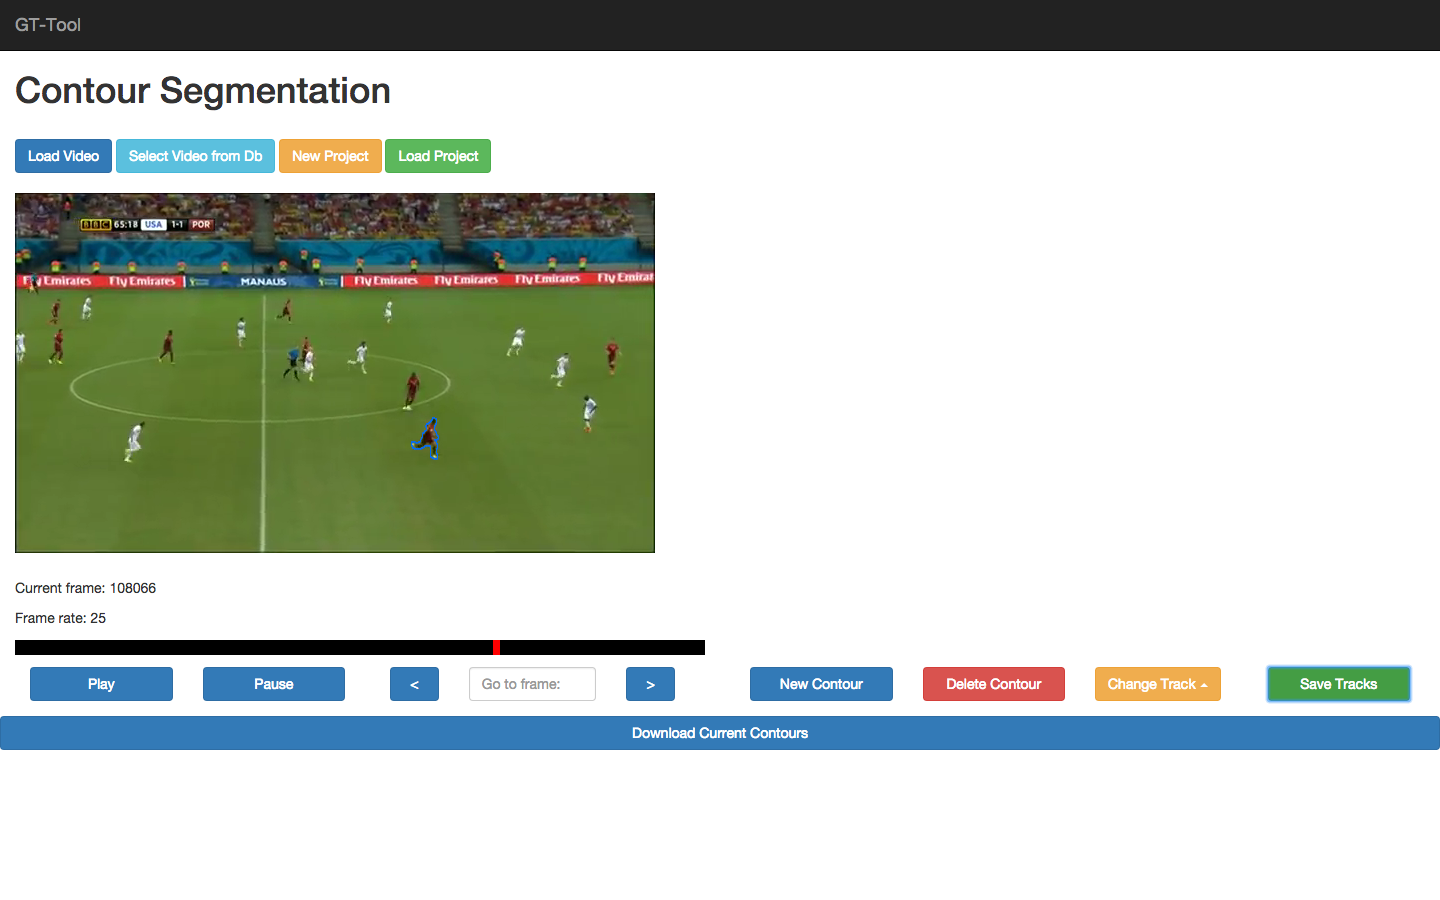
\includegraphics[width=\linewidth]{images/contourFull}
	\caption{Interfaz de segmentación de contornos completa} \label{fig:contourFull}
\end{figure}


\begin{figure}
	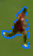
\includegraphics[width=0.2\linewidth]{images/contour1}
	\caption{Contorno de un jugador. Incluye todos los pixeles que conforman el contorno.} \label{fig:contour1}
\end{figure}


\subsection{Interfaz de segmentación semántica}

Finalmente se tiene el último modo de operación que es el de segmentación semántica. Esta interfaz es muy similar a la de segmentación temporal (como se puede apreciar en la Figura \ref{fig:semanticFull}), ya que en estos dos modos de operación el espacio de importancia es el tiempo. Al ser humano no le interesa tanto conocer las posiciones en $x$ o $y$ de los elementos en este modo de operación ya que la información semántica es obtenida a partir de método empíricos como la experiencia o la intuición. Lo que es relevante es que al presenciar cierto evento, se pueda capturar el inicio y final del mismo, y agregar una o más palabras clave que ayuden a clasificar el contenido. Por está razón la interacción de la interfaz del usuario se definió como se ve en la Figura \ref{fig:semantic1}.\\

Se puede observar que la acción que se le solicita al usuario es que presione los botones estando en el cuadro apropiado. Una vez que se utilizan botón de primer cuadro y último cuadro para fijar estos parámetros de correctamente solo hace falta introducir palabras clave separadas por espacios, que describan el contenido, las acciones o eventos que estén sucediendo en el video en un determinado momento. De esta manera se puede definir un período finito de tiempo con identificadores semánticos.\\

En la Figura \ref{fig:semantic2} se aprecia como son visualizados los datos semánticos previamente introducidos en la aplicación. Funciona de manera similar al modo de operación para segmentación temporal. Cada etiqueta posee dos botones, uno lo lleva al momento de inicio del evento, y el otro borra el evento de la base de datos.\\

\begin{figure}
	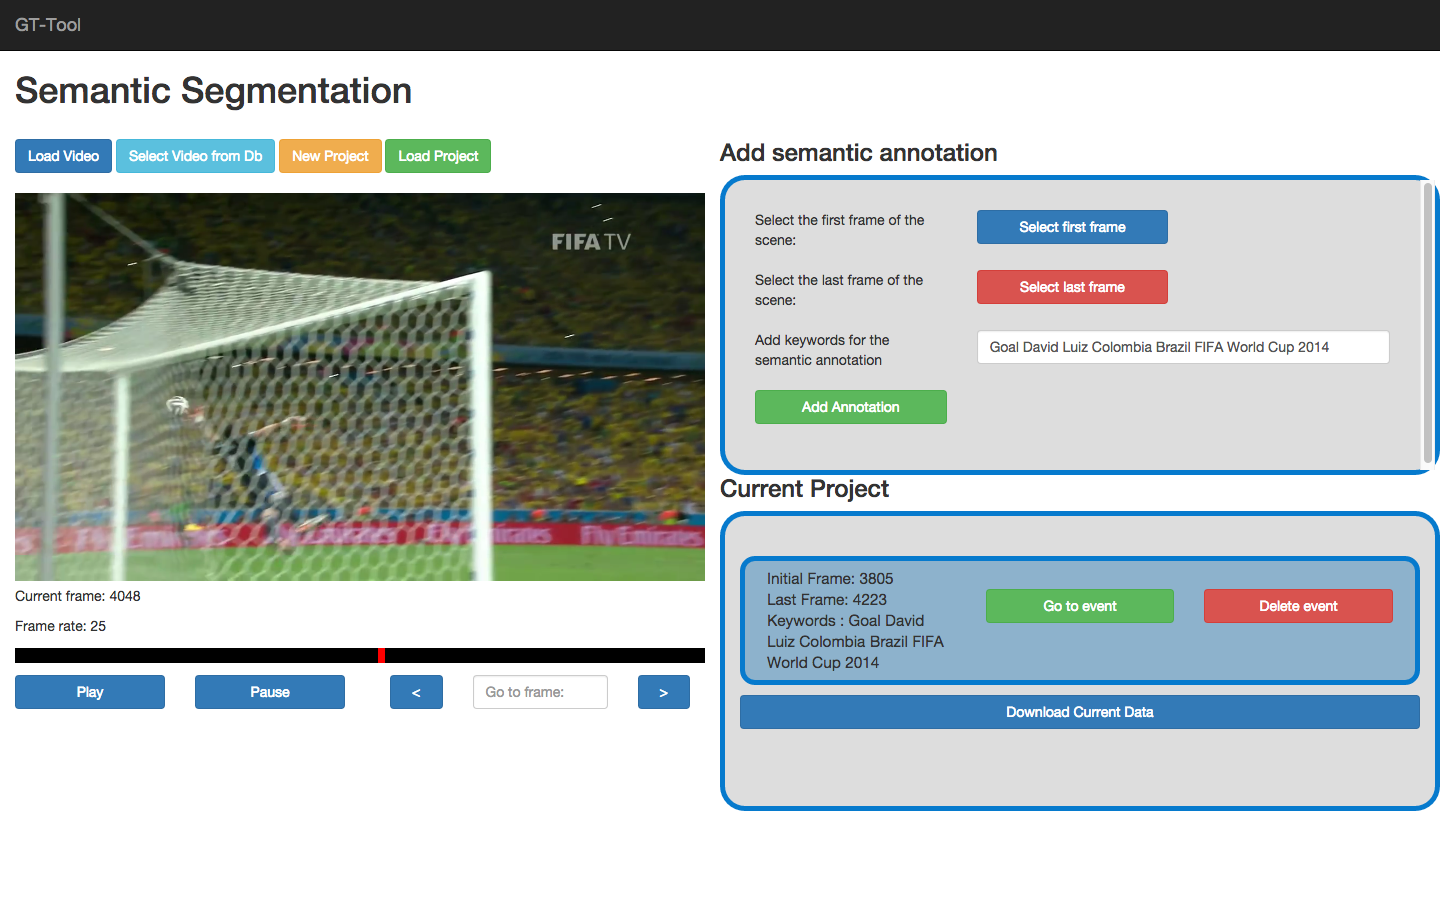
\includegraphics[width=\linewidth]{images/semanticFull}
	\caption{Interfaz de segmentación semántica completa} \label{fig:semanticFull}
\end{figure}

\begin{figure}
	
	\centering
	\begin{subfigure}[b]{0.7\textwidth}
		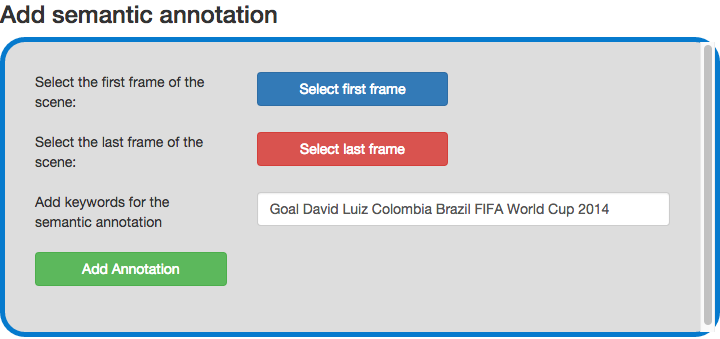
\includegraphics[width=\textwidth]{images/semantic1}
		\caption{Menu para agregar segmentaciones semánticas}
		\label{fig:semantic1}
	\end{subfigure}
	~ %add desired spacing between images, e. g. ~, \quad, \qquad, \hfill etc. 
	%(or a blank line to force the subfigure onto a new line)
	\begin{subfigure}[b]{0.7\textwidth}
		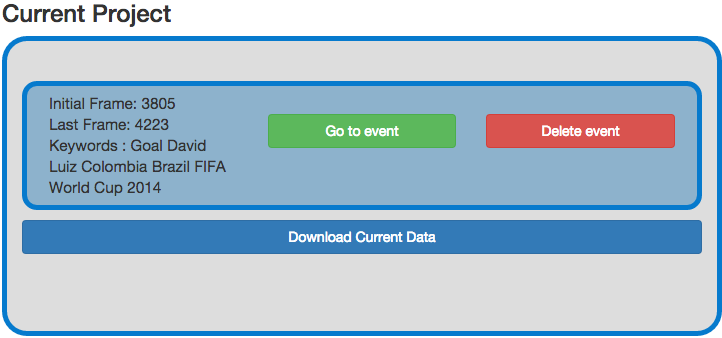
\includegraphics[width=\textwidth]{images/semantic2}
		\caption{Visualizador de segmentaciones semánticas actuales}
		\label{fig:semantic2}
	\end{subfigure}
\end{figure}

De esta manera se da por concluido el desarrollo de todos los modos de operación de la aplicación y como se ven y se utilizan sus respectivas interfaces.

\section{Backend}

Para el desarrollo del backend se utilizó la herramienta LoopBack. Esta provee una serie de funcionalidades genéricas para escribir y leer de bases de datos. Para configurar la herramientas e utilizan diferentes archivos JSON con los diferentes parámetros que definen el tipo de base de datos que se va a utilizar, las colecciones, y el modelo de los documentos. Los archivos .json de configuración se puede ver en la sección \ref{ap1} de los apéndices.\\

Una vez se hayan creado los archivos de configuración necesarios para tener cada una de las colecciones funcional, lo que se obtiene es un conjunto de métodos genéricos como los que se observan en la Figura \ref{fig:API}. Estos son diferentes tipos de métodos que se utilizan en las peticiones HTTP para realizar labores distintas. Lo métodos que se utilizaron en cada una de las colecciones fueron únicamente los POST, PUT, GET de la dirección raíz del servicio. Por ejemplo: un POST  a la dirección http:app@domain.com/api/contourSegmentation crearía un nuevo proyecto del tipo segmentación de contornos. Dichos métodos son suficientes para poder administrar correctamente lecturas y escrituras básicas a la base de datos. \\

Además de tener estos métodos genéricos, se puede tener métodos personalizados. Son desarrollados como si fuera un método del framework de NodeJS. Se creó un método especializado que puede ser utilizado por el administrador. Cuando este método se ejecuta, la función que realiza es escanear el directorio de videos dentro de la raíz del servidor, encuentra los archivos del tipo .mp4 y actualiza la base de datos para que dichos videos puedan estar disponibles para cargar desde el menu de carga desde el servidor remoto.\\

Finalmente la única configuración importante de cada uno de los modos de operación existentes que hace falta es la del modelo de los datos, es decir, como se ordena la información de cada uno de los documentos de la base de datos para que cada uno de ellos sea leído he interpretado de la manera correcta. Se tienen cuatro tipos específicos de modelo de datos y una forma general de como se almacenan los proyectos en la base de datos. Esto se explica con mayor detalle en la próxima sección que está dedicada a la base de datos.


\begin{figure}
	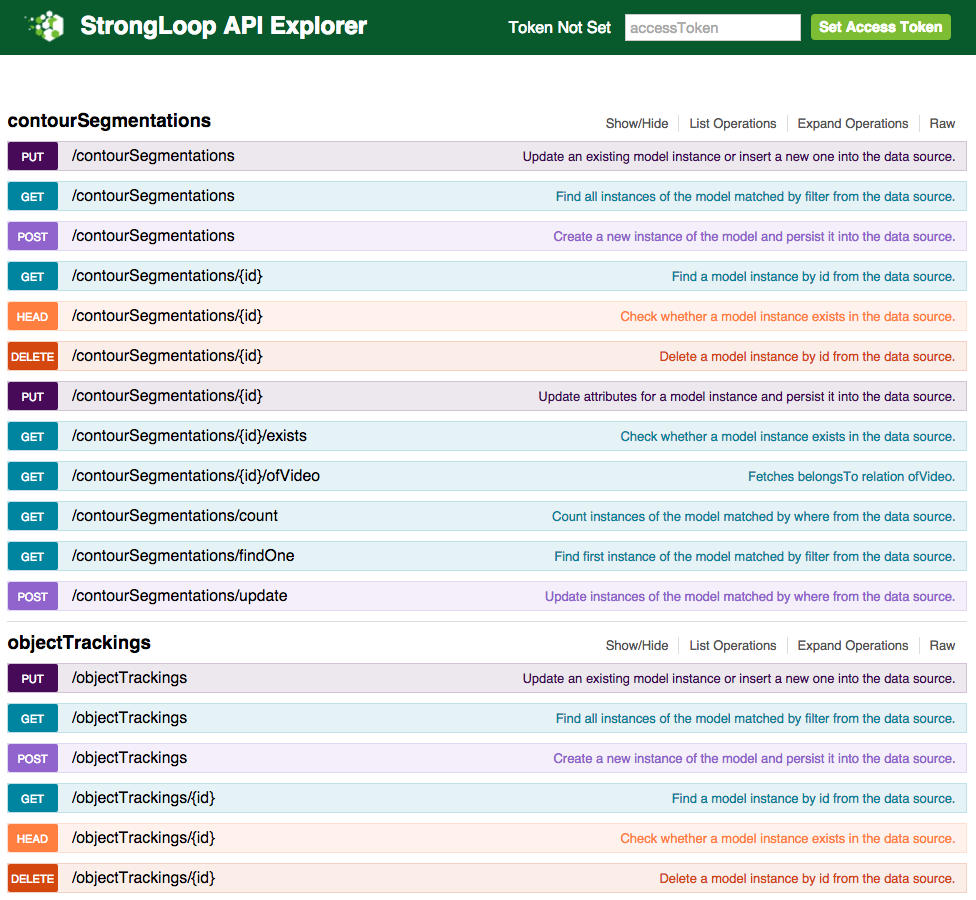
\includegraphics[width=\linewidth]{images/api}
	\caption{Visualización gráfica de los métodos del API} \label{fig:API}
\end{figure}

\section{Base de datos}


El diseño de la base de datos toma en cuenta cada uno de los diferentes modos de operación de la aplicación , por lo que se diseñó un tipo diferente de colección para cada uno de ellos. Todos los modos de operación tienen como base la estructura siguiente:

\begin{itemize}
\item \textit{id:} identificador único de la base de datos con el que se puede acceder a un documento. Es un número único en toda la colección para cada proyecto.
\item \textit{title:} variable en la cual se almacena el nombre del proyecto para luego poder cargarlo con facilidad, recordándolo por nombre.
\item \textit{author:} variable en la cual se almacena el autor del proyecto. 
\item \textit{data:} Es la información relevante de la segmentación realizada. Dependiendo del tipo de modo de operación, es la porción del documento de la base de datos que varía. Cada uno de los diferentes tipos se explican a continuación.
\end{itemize}

Como se observa la Figura \ref{fig:dbAr1}, todos los diferentes tipos de segmentación utilizan la misma estructura de proyecto. Lo que varía dentro de cada uno de ellos es la estructura del objeto denominado como \emph{data}. Las siguientes subsecciones se encargan de explicar el porqué de esta estructura.

\subsection{\textit{Data} en segmentación temporal}

En el caso de la segmentación temporal los datos relevantes son: cuadro inicial de una transición, cuadro final de una transición, el tipo de transición que ocurrió y el tipo de escena a la cual se llega luego de la transición. Por esta razón tiene el modelo de \emph{data} más sencillo de los cuatro modos de operación. Está compuesto por un arreglo de objetos donde los objetos tienen la siguiente estructura:\\

\textit{timeline data} = \{``initialFrame'',``lastFrame'',``eventType'',``sceneType''\}

\subsection{\textit{Data} en trayectorias de objetos}

Para este caso la información relevante es: cuadro actual, posición en X y posición en Y del centro del objeto en cada cuadro. Además a diferencia del modo de segmentación temporal, se puede tener más de un dato en el mismo período de tiempo, ya que durante cierto cuadro, pueden estar presentes dos o más objetos, a los cuales se debe de seguir de manera independiente. Por esta razón la estructura del dato es un poco más compleja y se puede observar como se compone en la Figura \ref{fig:dbAr1}.\\

Primero se asigna un nombre a la trayectoria, se le asigna un color específico que es con el que se van a visualizar las trayectorias en el video, y finalmente el apartado de data. En este se almacena un objeto que tiene tres partes, el número de cuadro de la posición en estudio, y las posiciones en $x$ y en $y$ del objeto. De esta manera se puede saber a cual objeto pertenece, donde está y en que instante de tiempo. Finalmente se puede representar como un objeto JSON de la siguiente manera:\\

\textit{track data} = \{``trackName'',``color'',``data''\}, donde data vendría dado por un arreglo de arreglos como el siguiente:\\

\textit{data} = [frameNumber,\{``xPosition'', ``yPosition''\}]

\subsection{\textit{Data} en segmentación espacial}

De manera muy similar se define el tipo de modelo para la segmentación de contornos. En este caso se aumentó un poco más el nivel de complejidad, ya que que los contornos no tienen únicamente una posición $x$ y $y$ como la posición, sino que más bien pueden tener N número de puntos. Por esta razón se extiende un poco más la profundidad del modelo y se hace un arreglo de objetos del tipo posición = \{``xPosition'',``yPosition''\} y finalmente se tiene la siguiente estructura, como se puede corroborar además en la Figura \ref{fig:dbAr1}:\\

\textit{contour data} = \{``contourName'',``color'',``contour information''\}\\

\textit{contour information} = [[``frameNumber'', ``contourPoints'' ]]\\

\textit{contourPoints} = [point0, ... , pointN],  donde pointX = \{``xPosition'',``yPosition''\}\\

\subsection{\textit{Data} en segmentación semántica}

Finalmente para la segmentación temporal se adopta un modelo muy similar al de la segmentación temporal, ya que no puede haber más una escena en el mismo espacio de tiempo, lo que se puede hacer es asignar una mayor cantidad de palabras clave al mismo segmento. El modelo para este tipo de segmentación queda definido de la siguiente manera:\\

\textit{semantic data} = \{``initialFrame'',``lastFrame'', keywords\}\\

\textit{keywords} = [``keyword0'', ..., ``keywordN'']\\


De esta manera se concluyen los cuatro tipos de modelos de la base de datos para los diferentes modos de operación según el tipo de segmentación que se quiera realizar.\\

Con esto se concluye el desarrollo de la aplicación y se continua con el análisis de resultados.

\begin{figure}
	\includegraphics[width=0.9\linewidth]{images/dbArq}
	\caption{Esquema del diseño de los modelos de la base de datos} \label{fig:dbAr1}
\end{figure}